\documentclass{beamer}
\beamertemplatenavigationsymbolsempty
\usepackage{amsmath, amssymb, hyperref, graphics}
\usepackage{tikz}
%\usepackage{mathpazo}
\usetikzlibrary{graphs}
\usetikzlibrary{graphs.standard}


\newcommand{\Z}{\mathbb{Z}}
\newcommand{\Q}{\mathbb{Q}}
\newcommand{\R}{\mathbb{R}}


\begin{document}
\begin{frame}{Instant Insanity / The Four Cubes Problem}

\begin{center}
  \includegraphics[width=.8\textwidth]{Pictures/InstantInsanityPackage.JPG}  
\end{center}
    \begin{itemize}
    \item Four cubes
    \item Each face coloured one of four colours: blue, green, red, yellow
    \item Arrange the cubes in a line so that each of the four long rows has one of each colour
\end{itemize}

\end{frame}
\begin{frame}{Prove the following set of cubes has no solution:}
\includegraphics[width=\textwidth]{Pictures/ImpossibleCubes.png}
\begin{block}{Not clear how to use graph theory....}
   ...make a graph that encodes which faces are \emph{opposite} each other on each cube.
  \end{block}

\end{frame}  

\begin{frame}{The four cubes encoded in a labelled graph}
\begin{center}
  \includegraphics[width=.7\textwidth]{Pictures/InstantInsanityImpossibleGraph.png}
\end{center}

\begin{block}{What would a solution look like in terms of the graph?}
 Consider front/back of cube first...
  
\end{block}

\end{frame}


\begin{frame}{A solution gives a certain pair of subgraphs...}
  \begin{block}{Looking at the edges encoding front/back of cubes}
    \begin{enumerate}
    \item One edge with each label in $\{1,2,3,4\}$
    \item Each vertex has degree two
    \end{enumerate}
  \end{block}
 Exactly the same with the edges encoding top/bottom of cubes.

 \begin{block}{Key fact:}
   A solution to Instantity Insanity gives a pair of subgraphs satisfying 1+2, and the subgraphs have with \emph{disjoint edges}.
  \end{block}

 \begin{block}{Can also go from a pair of subgraphs to a solution}
But slightly subtly, there might be several ways to do this: for each edge, need to \emph{choose} which colour is in front and which is in back...
 \end{block}
 
\end{frame}


\begin{frame}{Basic graphs and concepts}
  \begin{itemize}
  \item The \emph{empty graph} $E_n$ has $n$ vertices and no edges
  \item The \emph{complete graph} $K_n$ has $n$ vertices, and each vertex is connected to every other.
  \item The \emph{path graph} $P_n$ has $n$ vertices $\{1,\dots,n\}$ with an edge between $i$ and $i+1$
    \item The \emph{cycle graph} $C_n$ has $n$ vertices $\{1,\dots, n\}$ with an edge between $i$ and $i+1$ and between $n$ and $1$.

  \end{itemize}

\begin{definition}Let $G$ be a simple graph with vertex set $V$.  Its \emph{complement} $G^c$ is another graph with vertex set $V$, where two vertices $v,w\in V$ are adjacent in $G^c$ if and only if they are not adjacent in $G$. \end{definition}
  
\end{frame}

\begin{frame}{Obligatory Petersen graph}
  \begin{center}
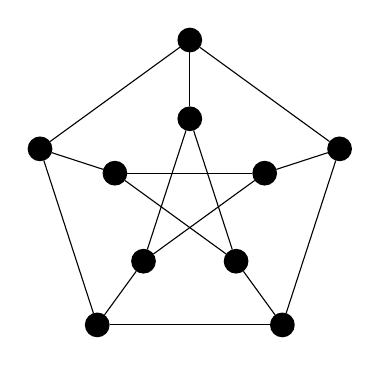
\begin{tikzpicture}[every node/.style={circle, draw, fill=black, inner sep=0pt, minimum width=4pt, thick}]
  \graph[clockwise, radius=2cm] {subgraph C_n [n=5,name=A]};
  \graph[clockwise, radius=1cm] {subgraph I_n [n=5,name=B]};

  \foreach \i in {1,2,3,4,5}{\draw (A \i) -- (B \i);}
  \newcounter{j}
  \foreach \i in {1,2,3,4,5}{%
  \pgfmathsetcounter{j}{ifthenelse(mod(\i+2,5),mod(\i+2,5),5)}
  \draw (B \i) -- (B \thej);
  }
\end{tikzpicture}
\end{center}
\end{frame}

\begin{frame}[plain,c]

\begin{center}

\Huge

\usebeamercolor[fg]{frametitle}
What does it mean for a graph to be connected?
\end{center}

\end{frame}


\begin{frame}{Connected means we can ``get from any vertex to another''}
  \begin{definition}[Walk] Let $G$ be a simple graph.  A \emph{walk} in $G$ is a sequence of vertices $v_1, v_2, \dots, v_n$ so that $v_i$ is adjacent to $v_{i+1}$.  We we say the walk goes from $v_1$ to $v_n$.
    \end{definition}

  \begin{definition}[Connected] A graph $G$ is \emph{connected} if there is a walk between any two vertices $v$ and $w$ in $G$.
  \end{definition}

  \begin{block}{Definitions I won't use without explaining}
    \begin{itemize}
    \item A \emph{trail} is a walk that doesn't repeat any edges
    \item A \emph{path} is a walk that doesn't repeat any vertices
    \end{itemize}
    \end{block}

\end{frame}
  
\begin{frame}{Bipartite graphs}
  \begin{definition}[Bipartite graphs] A graph $G$ is \emph{bipartite} if we can colour every vertex either blue or red so that every edge goes between a blue vertex and a red vertex.
  \end{definition}
  \begin{definition}[Complete bipartite graphs] The \emph{complete bipartite graph} $K_{m,n}$ consists of $m+n$ vertices, $m$ coloured red, $n$ coloured blue, and an edge between any red vertex and and any blue vertex.
  \end{definition}

  \begin{block}{Examples}
    \end{block}
\end{frame}

\begin{frame}{Another way to characterise bipartite graphs}  
  \begin{lemma}A graph $G$ is bipartite if and only if it doesn't have any cycles of odd length (i.e., subgraphs of the form $C_{2k+1}$).
    
    \end{lemma}
  \begin{block}{Bipartite $\implies$ no odd cycles:}
    Subgraphs of bipartite graphs are bipartite
  \end{block}
  \begin{block}{No odd cycles $\implies$ Bipartite:}
Try to colour $G$ by distance from $v$   
\end{block}
  \begin{definition}[Distance]Let $G$ be connected, and let $v,w$ be two vertices.  The \emph{distance from $v$ to $w$} is the least number of edges in any walk from $v$ to $w$.
    \end{definition}


  
\end{frame}






\end{document}
